%%%%%%%%%%%%%%%%%%%%%%%%%%%%%%%%%%%%%%%%%%%%%%%%%%%%%%%%%%%
\section{About research}
%%%%%%%%%%%%%%%%%%%%%%%%%%%%%%%%%%%%%%%%%%%%%%%%%%%%%%%%%%%
%
%
%%%%%%%%%%%%%%%%%%%%%%%%%%%%%%%%%%%%%%%%%%%%%%%%%%%%%%%%%%%
\subsection{A typical scientific lab}
%%%%%%%%%%%%%%%%%%%%%%%%%%%%%%%%%%%%%%%%%%%%%%%%%%%%%%%%%%%
%
%
\begin{frame}[t, negative]
	\subsectionpage
\end{frame}
%
%
\begin{lhframe}[rhgraphic={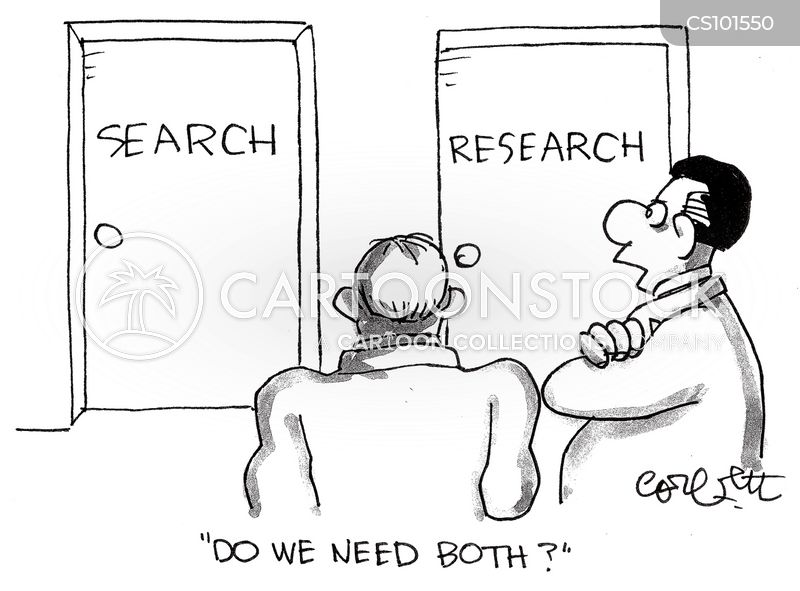
\includegraphics[scale=0.32]{lab1.jpg}}]
	{A typical scientific lab\footnote{\citet{McElreath_2020}, lecture $20$ and \citet{McElreath_2022}, chapter $17$ \nocite{McElreath_2019} \nocite{Hernan_et_al_2020} \nocite{Cunningham_2022} } }
	
	What is needed? \\
	
	\begin{enumerate}
		%
		\item Quality of theory
		\item Quality of data
		\item Reliable procedures and code
		\item Quality of data analysis
		\item Documentation
		\item Reporting
		%
	\end{enumerate} 
	%
\end{lhframe}
%
%
\begin{lhframe}[rhgraphic={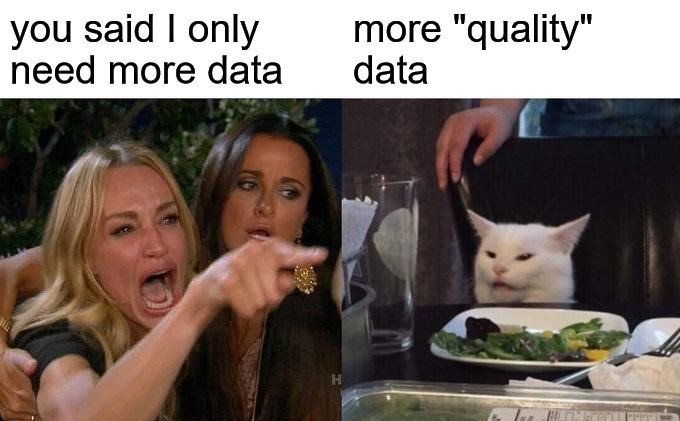
\includegraphics[scale=0.41]{woman_cat.jpg}}]
	{A typical scientific lab}
	
	What we ``normally" focus on? \\
	
	\begin{enumerate}
		%
		\item \textcolor{blue}{Quality of theory}
		\item \textcolor{blue}{Quality of data}
		\item Reliable procedures and code
		\item \textcolor{blue}{Quality of data analysis}
		\item Documentation
		\item Reporting
		%
	\end{enumerate}
	%
\end{lhframe}
%
%
\begin{lhframe}[rhgraphic={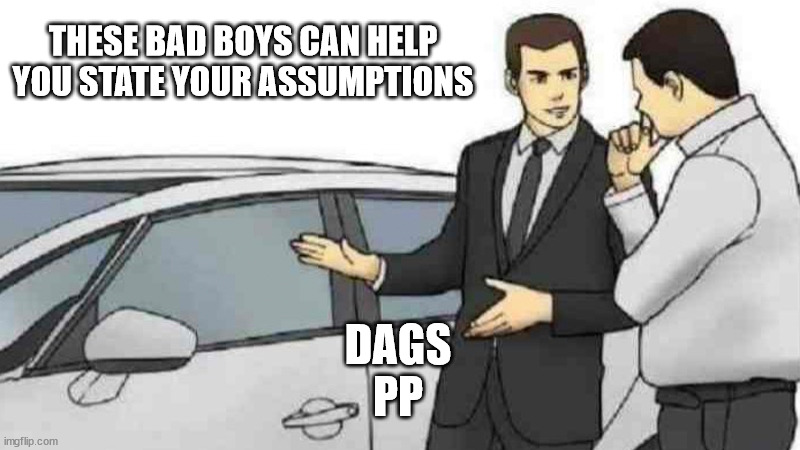
\includegraphics[scale=0.25]{car_salesman.jpg}}]
	{A typical scientific lab}
	
	What can be improved?\footnote{see \citet{Yarkoni_2020} on a discussion on how the failure in alignment between verbal and statistical expressions is related to psychology's replication crisis.}\\
	{\small (with DAGs and PP)}
	\begin{enumerate}
		%
		\item \textcolor{blue}{Quality of theory}
		\item \textcolor{blue}{Quality of data}
		\item \alert{Reliable procedures and code}
		\item \textcolor{blue}{Quality of data analysis}
		\item \textcolor{blue}{Documentation}
		\item Reporting
		%
	\end{enumerate}
	%
\end{lhframe}
%
%
%%%%%%%%%%%%%%%%%%%%%%%%%%%%%%%%%%%%%%%%%%%%%%%%%%%%%%%%%%%
\subsection{Research hypothesis production}
%%%%%%%%%%%%%%%%%%%%%%%%%%%%%%%%%%%%%%%%%%%%%%%%%%%%%%%%%%%
%
%
\begin{frame}[t, negative]
	\subsectionpage
\end{frame}
%
%
\begin{lhframe}[rhgraphic={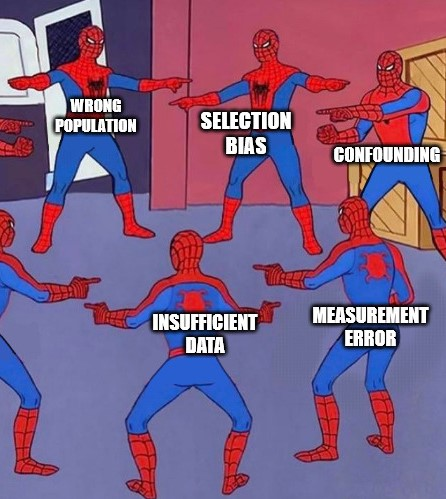
\includegraphics[scale=0.5]{challenges.jpg}}]
	{Research hypothesis production}
	
	Well known challenges\footnote{\citet{Hernan_2020}, lesson $4$}
	%
	\begin{itemize}
		%
		\item Insufficient data
		\item Wrong population
		\item Measurement error
		\item Selection bias
		\item Confounding
		%
	\end{itemize} 
	%
\end{lhframe}
%
%
\begin{lhframe}[rhgraphic={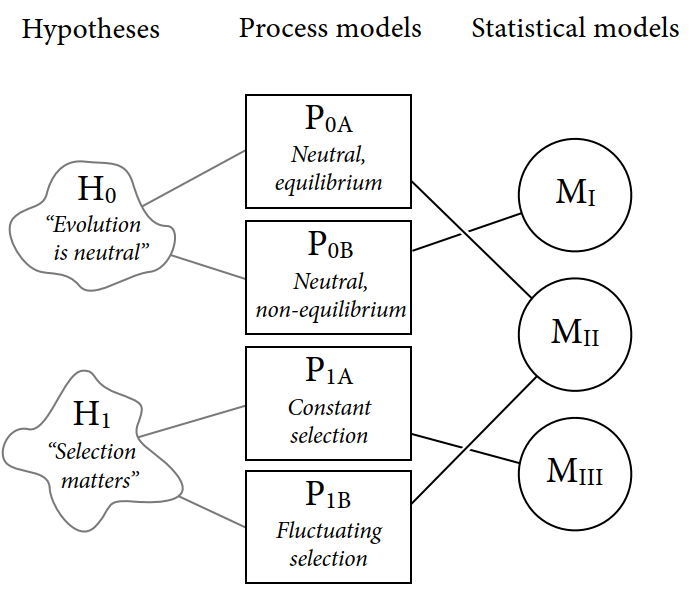
\includegraphics[scale=0.45]{process_models.png}}]
	{Research hypothesis production}
	
	but we should not forget\footnote{Figure 1.2 reproduced from chapter $1$ \citet{McElreath_2022}}
	%
	\begin{itemize}
		%
		\item No one-to-one relationship exists between our \textcolor{blue}{process models} and \textcolor{blue}{statistical models},
		%
		\item Nor between our hypothesis and a process models
	\end{itemize} 
	%
\end{lhframe}
%
%
\begin{lhframe}[rhgraphic={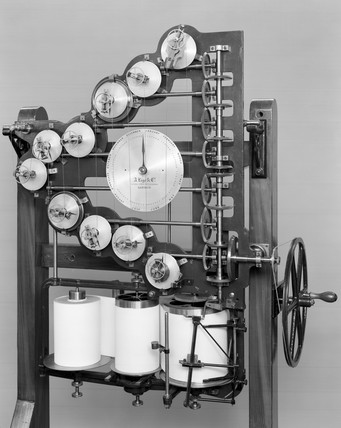
\includegraphics[scale=2.5]{tide_machine.jpg}}]
	{Research hypothesis production}
	
	and also
	%
	\begin{itemize}
		%
		\item \textcolor{blue}{statistical models} are just \textcolor{blue}{``machines to find association"}, not a reliable reflection of the theory \\
		\alert{(I can prove it!!)}.
		%
	\end{itemize} 
	%
\end{lhframe}
%
%
\begin{lhframe}[rhgraphic={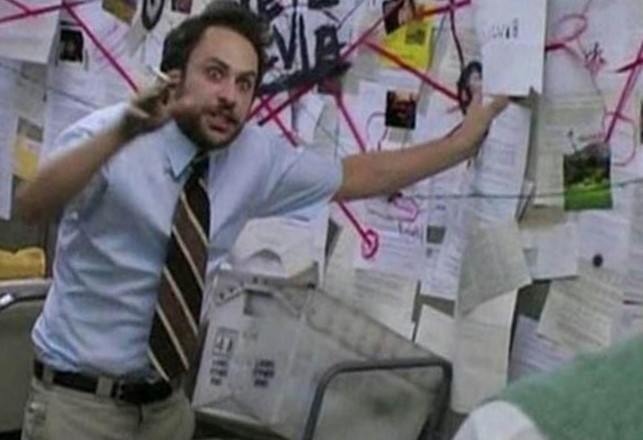
\includegraphics[scale=0.55]{lab2.jpg}}]
	{Research hypothesis schematics\footnote{\citet{McElreath_2022}, lecture $20$, \citet{Pearl_2019}. Follow \citet{Fogarty_et_al_2022} on item (c).}}
	
	\begin{enumerate}
		%
		\item[a.] Estimand and \textcolor{blue}{process model}
		\item[b.] Synthetic data generation
		\item[c.] Statistical model design and testing
		\item[d.] Apply \textcolor{blue}{statistical model} to data 
		%
	\end{enumerate} 
	%
\end{lhframe}
%
%
\begin{lhframe}[rhgraphic={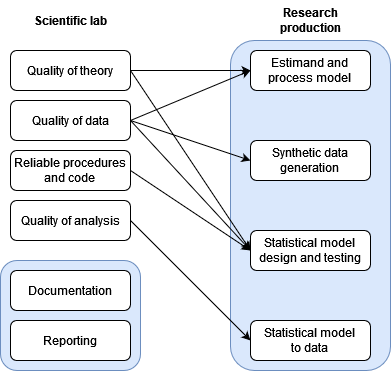
\includegraphics[scale=0.42]{lab_to_research.png}}]
	{Research hypothesis schematic}
	
	Where does it match with the previous?
	%
	\begin{enumerate}
		%
		\item[a.] Estimand and process model\\
		\small{maps \textcolor{blue}{1 (theory)} and \textcolor{blue}{2 (data)} to a heuristic model.}
		%
		\item[b.] Synthetic data generation \\
		\small{maps \textcolor{blue}{2 (data)} to an idealized data.}
		%
		\item[c.] Statistical model design and testing \\
		\small{maps \textcolor{blue}{1 (theory)}, \textcolor{blue}{2 (data)}, and \textcolor{blue}{3 (reliable code)} to an statistical model.}
		%
		\item[d.] Apply statistical model to data \\
		\small{maps \textcolor{blue}{4 (analysis)} onto a result.}
		%
	\end{enumerate} 
	%
\end{lhframe}
%
%
\begin{lhframe}[rhgraphic={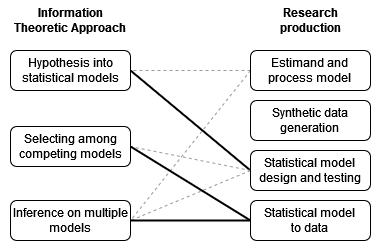
\includegraphics[scale=0.62]{ITA_to_research.png}}]
	{Where does the ITA fit?}
	
	Information Theoretic Approach (ITA) is framework to select among competing models \cite{Anderson_2008, Chamberlain_1965}:
	%
	\begin{enumerate}
		%
		\item Hypothesis into statistical models, \\
		{\small \alert{(how about a process model?)} }
		%
		\item Select among competing models,  \\
		{\small \alert{(do the code works as intended?)} }
		%
		\item Make inferences based on one or multiple models. \\
		{\small \alert{(do the code works as intended?, \\
				are there variables that can bias our results?)} }
		%
	\end{enumerate}
	%
\end{lhframe}
%
%